% nla-groot — Mechanistic Interpretability Workshop (NeurIPS 2026 target).
% Short paper: max 4 pages + references (check CFP when OpenReview opens).
%
% Build:  make -C paper
% Before submit: swap in the official workshop style file from the CFP pack;
% scrub author strings, repo URLs, and paths from the PDF.

\documentclass[10pt]{article}

\usepackage[letterpaper, margin=0.85in]{geometry}
\usepackage[utf8]{inputenc}
\usepackage[T1]{fontenc}
\usepackage{lmodern}
\usepackage{microtype}
\usepackage{amsmath,amssymb}
\usepackage{graphicx}
\usepackage{booktabs}
\usepackage{multirow}
\usepackage[numbers,sort&compress]{natbib}
\usepackage[colorlinks=true,linkcolor=black,citecolor=blue!50!black]{hyperref}
\usepackage{url}
\usepackage{tikz}
\usetikzlibrary{positioning,arrows.meta}
\usepackage{enumitem}
\setlist{nosep,leftmargin=*}

\graphicspath{{figures/}}

\newcommand{\AV}{\ensuremath{\mathrm{AV}}}
\newcommand{\AR}{\ensuremath{\mathrm{AR}}}
\newcommand{\hvec}{\mathbf{h}}
\newcommand{\hhat}{\hat{\mathbf{h}}}
\newcommand{\code}[1]{\texttt{\small #1}}
\sloppy

\title{When Reconstruction Passes:\\
  Natural-Language Autoencoders on VLA Activations\\
  Fail Grounding and Semantic Steering}

\author{Anonymous Author(s)}

\date{}

\begin{document}
\maketitle

\begin{abstract}
Natural-language autoencoders (NLAs) map neural activations to text and back,
offering readable interfaces to model internals.
We port the NLA recipe to the GR00T vision-language-action (VLA) backbone:
extract per-token hidden states, train an activation verbalizer (\AV) and
reconstructor (\AR), and inject \AR{} outputs as live backbone steers in
LIBERO simulation.
Supervision uses a multimodal \emph{teacher} (frames + instruction), not
human descriptions of what \(\hvec\) encodes---a confound inherited from the
original LLM setting.
We release \code{nla-groot} and a three-axis evaluation protocol:
(1)~offline reconstruction and retrieval,
(2)~vision-grounded caption judging,
(3)~closed-loop steer A/B (matched vs.\ mismatched language).
On our main checkpoint, reconstruction metrics pass while grounding,
anti-template specificity, and semantic steering fail.
\textbf{Claim:} NL autoencoders on VLA activations are misleading without
vision-grounded and behavioral checks---use this protocol before trusting
captions or steering policies with language.
\end{abstract}

\section{Introduction}
\label{sec:intro}

Vision-language-action policies such as GR00T~\citep{nvidia2025gr00t} couple a
multimodal backbone to a diffusion action head.
The backbone hidden state \(\hvec \in \mathbb{R}^{2048}\) at layer~16 is
causally upstream of actions, yet there is no standard way to read or write
\(\hvec\) in natural language.
\citet{frasertaliente2026nla} propose \emph{natural-language autoencoders}:
\(\AV(\hvec)\) produces a caption and \(\AR(y)\) reconstructs
\(\hhat \approx \hvec\), yielding both an interpretability artifact and a
causal handle for activation steering~\citep{turner2023actadd,zou2023repe}.

We ask whether this recipe \emph{transfers} to a VLA backbone, where
(i)~activations are multimodal and task-conditioned,
(ii)~downstream \emph{behavior} is the right falsification test, and
(iii)~training labels are \textbf{synthetic}: a GPT-class teacher sees camera
frames and token metadata, \emph{not} raw \(\hvec\) floats.
The teacher may describe scene attributes only weakly present in \(\hvec\);
supervised fine-tuning (SFT) therefore optimizes
\(P(\text{teacher text} \mid \hvec)\), not faithful ``what \(\hvec\) means.''

\paragraph{Contribution.}
We do not claim a strong \AV{} or working semantic steer.
We claim a \textbf{negative, actionable result}:
autoencoder metrics can look successful while captions are
vision-ungrounded and steering is behaviorally non-semantic.
We release open tooling and a pre-registered \textbf{three-axis scorecard}
so NLA ports on policies are not validated by reconstruction alone.

\begin{figure}[t]
  \centering
  \resizebox{\linewidth}{!}{% System overview figure for nla-groot.
% Solid arrows: training signal. Dashed arrows: inference / steering.
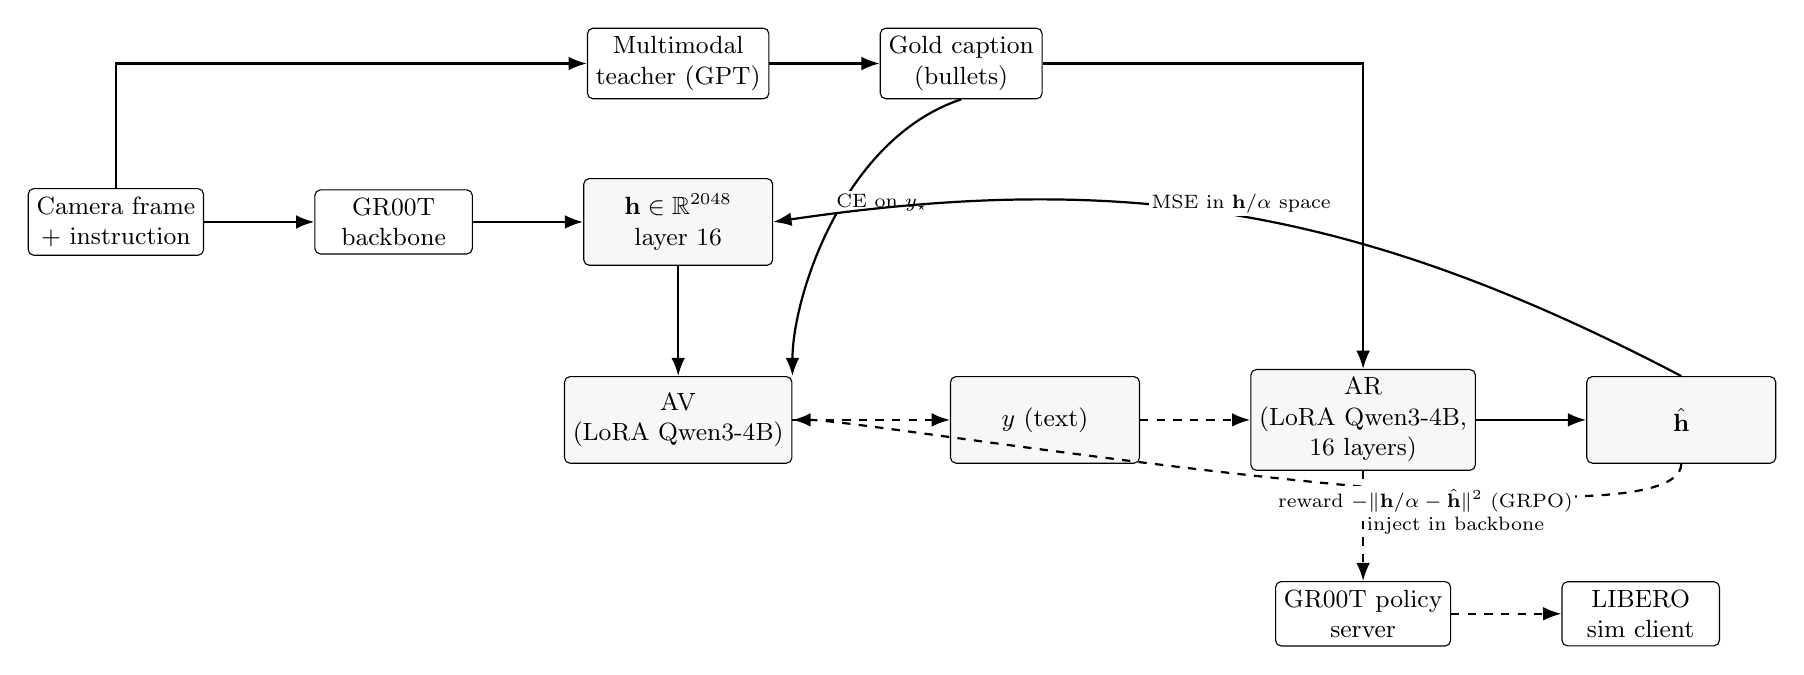
\begin{tikzpicture}[
    >=Latex,
    font=\small,
    node distance=10mm and 14mm,
    every node/.style={align=center},
    box/.style={rectangle, draw, rounded corners=2pt,
                minimum height=8mm, minimum width=20mm, align=center,
                inner sep=3pt},
    bigbox/.style={box, fill=black!3, minimum height=11mm,
                   minimum width=24mm},
    inflow/.style={->, thick},
    steerflow/.style={->, thick, dashed},
    lbl/.style={midway, font=\scriptsize, align=center,
                fill=white, inner sep=1pt}
  ]

  % Top row: extraction pipeline.
  \node[box]                       (frame)  {Camera frame\\+ instruction};
  \node[box, right=of frame]       (groot)  {GR00T\\backbone};
  \node[bigbox, right=of groot]    (h)      {$\hvec\in\mathbb{R}^{2048}$\\layer 16};

  % Teacher labeling above h.
  \node[box, above=of h]           (teacher){Multimodal\\teacher (GPT)};
  \node[box, right=of teacher]     (gold)   {Gold caption\\(bullets)};

  % AV and AR in the centre.
  \node[bigbox, below=14mm of h]   (AV)     {\AV{}\\(LoRA Qwen3-4B)};
  \node[bigbox, right=20mm of AV]  (text)   {$y$ (text)};
  \node[bigbox, right=of text]     (AR)     {\AR{}\\(LoRA Qwen3-4B,\\16 layers)};
  \node[bigbox, right=of AR]       (hhat)   {$\hhat$};

  % Down-stream: live policy server + sim.
  \node[box, below=14mm of AR]     (server) {GR00T policy\\server};
  \node[box, right=of server]      (sim)    {LIBERO\\sim client};

  % Extraction edges.
  \draw[inflow] (frame) -- (groot);
  \draw[inflow] (groot) -- (h);
  \draw[inflow] (frame.north) |- (teacher.west);
  \draw[inflow] (teacher) -- (gold);

  % Training: h -> AV; gold supervises AV (CE).
  \draw[inflow] (h.south) -| (AV.north);
  \draw[inflow] (gold.south) .. controls +(-1.5,-0.5) and +(0,1.0) ..
    (AV.north east) node[lbl, above right=1mm and 0mm] {CE on $y_\star$};

  % Training: gold -> AR -> hhat; MSE against h.
  \draw[inflow] (gold.east) -| (AR.north);
  \draw[inflow] (AR) -- (hhat);
  \draw[inflow, bend right=18] (hhat.north) to
    node[lbl, above] {MSE in $\hvec/\alpha$ space} (h.east);

  % AV -> text -> AR at inference (and AR-AV-mix during late SFT).
  \draw[steerflow] (AV) -- (text);
  \draw[steerflow] (text) -- (AR);

  % Steering: AR -> server -> sim.
  \draw[steerflow] (AR.south) -- (server.north)
    node[lbl, right] {inject in backbone};
  \draw[steerflow] (server) -- (sim);

  % Optional GRPO loop: AR is the reward.
  \draw[steerflow] (hhat.south) .. controls +(0,-1.2) and +(1,0) ..
    (AV.east) node[lbl, below right=1mm and 1mm]
    {reward $-\|\hvec/\alpha - \hhat\|^2$ (GRPO)};

\end{tikzpicture}
}
  \caption{\textbf{Pipeline.} Solid: training (\(\hvec\) from GR00T hook;
  gold captions from teacher).
  Dashed: inference (\(\hhat=\AR(y)\) steers the live policy).
  Auditing uses \(\AV(\hvec)\); steering bypasses \(\AV\).}
  \label{fig:pipeline}
\end{figure}

\section{Setup (minimal)}
\label{sec:setup}

\paragraph{Activations.}
A forward hook on GR00T \code{backbone\_features} (Qwen3-VL, layer~16,
pre-action-head LayerNorm) records \(\hvec_i\) per token at three position
types: \code{last\_text}, \code{image\_patch}, \code{anchor}.
Corpus: LIBERO Goal/Spatial/Object/10 LeRobot trajectories;
\(\alpha \approx \) P75\(\|\hvec\|_2\) for injection scaling.

\paragraph{\AV{} and \AR{}.}
Both are LoRA~\citep{hu2022lora} fine-tunes of Qwen3-4B-Instruct.
\AV{} injects \(\alpha\cdot\mathrm{normalize}(\mathbf{W}_p\hvec)\) at a
reserved slot token and is trained with CE on teacher bullets.
\AR{} reads ``Summary of the following text:'' and predicts
\(\hhat/\alpha\); loss is MSE plus InfoNCE hard negatives.
Joint SFT (\code{libero\_4suite\_v3}: 15k steps, batch 4, optional
\code{ar\_av\_mix} to expose \AR{} to \AV{} samples).

\paragraph{Steering.}
At inference, user text \(y\) maps to \(\hhat=\AR(y)\) and blends into
backbone tokens (\code{image\_patch} or \code{image\_patch\_all}) on every
\code{get\_action} call in the official LIBERO policy server.

\section{Three-axis evaluation protocol}
\label{sec:protocol}

Each checkpoint is scored on \textbf{independent} axes; overall PASS requires
required metrics (pre-registered in \code{build\_v3\_scorecard.py}).

\paragraph{Axis 1: Reconstruction \& retrieval.}
Closed-loop cosine \(\cos(\hvec,\AR(\AV(\hvec)))\) without teacher forcing;
retrieval margin (matched vs.\ cross-pair \(\AR(\AV(\hvec))\)).
High scores mean \(\AV\) and \(\AR\) form a consistent codec---not that
language matches pixels.

\paragraph{Axis 2: Vision-grounded judge.}
\code{llm\_judge\_av\_captions.py} scores captions against \emph{cached frames}
(grounding / specificity; appropriateness for position type).
We report gold (teacher) vs.\ \(\AV\) greedy on identical rows; gold sets a
ceiling ($\sim$75--83\% grounding on held-out samples).

\paragraph{Axis 3: Closed-loop steer A/B.}
On \code{put\_the\_bowl\_on\_the\_plate} (LIBERO Goal, GR00T checkpoint,
seeds \(\{0,1,2\}\)): baseline, \emph{correct} steer text, \emph{wrong} text.
Primary metric: \(\Delta_{cw} = \mathrm{succ}_{\text{correct}} -
\mathrm{succ}_{\text{wrong}}\) (PASS if $\geq 5$pp).
Semantic steering requires \(\Delta_{cw} > 0\), not merely
\(\mathrm{succ} \neq \mathrm{succ}_{\text{baseline}}\).

\paragraph{Auditing (optional fourth arm).}
Counterfactual panel: baseline / edited / control \(\AV\) explanations under
\(\hvec\) edits (\code{run\_interp\_panel.py}) for hypothesis testing;
complements Axes~2--3.

\section{Results: metrics pass, semantics fail}
\label{sec:results}

Table~\ref{tab:scorecard} is the V3 scorecard (\textbf{overall FAIL}).
Retrieval margin \textbf{passes} (0.124 vs.\ 0.05 threshold); judge
anti-template specificity \textbf{fails} (8.3\% vs.\ 50\%);
\(\Delta_{cw}=0\) (WARN).

\begin{table}[t]
  \centering
  \caption{V3 scorecard (\code{libero\_4suite\_v3}). Required metrics
  gate overall verdict.}
  \label{tab:scorecard}
  \small
  \begin{tabular}{@{}lrrl@{}}
    \toprule
    Metric & Value & Thr. & Verdict \\
    \midrule
    retrieval\_margin & 0.124 & 0.05 & PASS \\
    judge\_grounding\_specific & 0.417 & 0.55 & WARN \\
    judge\_anti\_template & 0.083 & 0.50 & FAIL \\
    sim\_correct\_minus\_wrong & 0.000 & 0.05 & WARN \\
    \bottomrule
  \end{tabular}
\end{table}

\paragraph{Template collapse (Axis 2).}
Table~\ref{tab:judge}: on 4-suite holdout, gold grounding is 75\% but
\(\AV\) is 41.7\%; anti-template specificity drops from 50\% (gold) to
\textbf{8.3\%} (\(\AV\))---captions collapse to reusable scene templates
(``kitchen counter / green bowl'') across different tasks.
Appropriateness stays 100\% for \(\AV\): prose \emph{looks} valid while
being vision-wrong (\emph{shorthand collapse}).

\begin{table}[t]
  \centering
  \caption{Multimodal judge pass rates (24-row held-out sample).}
  \label{tab:judge}
  \small
  \begin{tabular}{@{}llrr@{}}
    \toprule
    Checkpoint & Source & Ground. & Anti-templ. \\
    \midrule
    \multirow{2}{*}{v3 (4-suite)}
      & gold & 0.750 & 0.500 \\
      & \(\AV\) & 0.417 & 0.083 \\
    \bottomrule
  \end{tabular}
\end{table}

\paragraph{Symmetric steering (Axis 3).}
Baseline solves all seeds (\(\mathrm{succ}=1.0\)).
Every steer arm fails (\(\mathrm{succ}=0\)) for both \emph{matching} and
\emph{contradictory} prompts---\(\Delta_{cw}=0\).
Bowl displacement $\approx$0.145\,m (baseline) vs.\ $\approx$0.07\,m (all
steers): intervention \emph{dampens} motion uniformly rather than redirecting
toward the prompted object.
\textbf{Steerability \(\neq\) faithful interpretability.}

\paragraph{Negative result in one line.}
Reconstruction and retrieval can certify a low-loss text--vector codec
while (i)~captions fail vision grounding and (ii)~language steers do not
separate correct from wrong instructions.

\section{Use this before you trust or steer}
\label{sec:conclusion}

\paragraph{For auditing.}
Do not treat \(\AV(\hvec)\) as ground truth without Axis~2 on held-out
frames and, when possible, counterfactual \(\hvec\) edits (Axis~4).
Report gold-vs-\(\AV\) gaps, not \(\AV\) alone.

\paragraph{For steering.}
Do not deploy \(\AR(y)\) backbone steers because reconstruction is high.
Require \(\Delta_{cw} > 0\) on held-out tasks and dose calibration;
until then, treat NL steers as \emph{unvalidated interventions}.

\paragraph{For training.}
Teacher-only SFT lacks an explicit pixel alignment term; reconstruction
rewards template IDs invertible by \(\AR\).
Mitigations we document but do not fully solve here: label QA,
quality-weighted SFT, mined hard negatives, judge-blended GRPO.

\paragraph{Reproducibility.}
Anonymous code: \url{https://anonymous.4open.science/} (placeholder---replace
before submit).
Scorecard: \code{scripts/eval/build\_v3\_scorecard.py};
commands: \code{paper/repro/canonical\_commands.sh}.

\section*{Broader impact}
NL interfaces to policy internals could help safety auditing or harm if
misread as faithful; our protocol is meant to reduce overclaim.

\bibliographystyle{unsrtnat}
\bibliography{refs}

\end{document}
